%Introductory text:
In this section, some basic concepts are introduced, concerning possibility theory, possibilistic variables and fuzzy numbers and intervals. The framework of set evaluation by ill-known constraints\cite{Pon11} is explained. The section concludes with a brief introduction to temporal databases.

\subsection{\label{subsec:possibility-theory}Possibility Theory}
Possibility theory, like probability theory, deals with uncertainty about the outcome of an experiment. In probability theory, this uncertainty is caused by the \emph{variability} in the outcomes, while in possibility theory, the uncertainty is caused by \emph{incomplete knowledge} about the experiment. The quantification of confidence in probability theory is achieved by means of a measure of chance, whereas in possibility theory, possibility and necessity measures are used. In any case, the quantification of confidence in a theory of uncertainty is achieved using a confidence measure\cite{Shafer:1976:AMathematical}.

\begin{definition}
Consider a set of outcomes $\Omega$. Let $\wp(\Omega)$ denote the powerset of $\Omega$ and let $A$ and $B$ be elements of $\wp(\Omega)$. A \emph{confidence measure on $\Omega$} is defined by a function
	\begin{align}
	g : \wp(\Omega) & \rightarrow \left[0,1\right]
	\end{align}
that satisfies
	\begin{align}
	g(\emptyset) &= 0 \\
	g(\Omega) &= 1 	\label{NormalizationProperty} \\
	A \subseteq B &\Rightarrow g(A) \leq g(B) \label{MonotonicityProperty}
	\end{align}
\end{definition}

Both possibility measures and necessity measures are special cases of confidence measures.

\begin{definition}
Consider a confidence measure $\Pi$ on a set of outcomes $\Omega$. Let $J$ be a countable index set and let $\{ A_{j} | j \in J \wedge A_{j} \subseteq \Omega \}$ be a family of elements of $\wp(\Omega)$. $\Pi$ is now a \emph{possibility measure on $\Omega$} if it satisfies:
	\begin{align}
	\Pi\left(\bigcup_{j \in J} A_{j} \right) = \sup_{j \in J} \Pi(A_{j})
	\end{align}
\end{definition}

In this work, the interpretation is as follows. The possibility of an event expresses how plausible the occurrence of the event seems to an observer of the experiment, given the (partial) knowledge of the observer about the experiment.

Information on the possibility of distinct elements of the universe of discourse $\Omega$ can now be given by a \emph{possibility distribution} $\pi$ on $\Omega$, defined by:

\begin{definition}
Consider a possibility measure $\Pi$ on $\Omega$. A \emph{possibility distribution} $\pi$ on $\Omega$ underlying the possibility measure $\Pi$ is then a function defined by:
	\begin{align}
	\pi : \Omega \rightarrow \left[0, 1\right] : \pi(u) = \Pi(\{u\})
	\end{align}
\end{definition}

\begin{definition}
Consider a confidence measure $N$ on a set of outcomes $\Omega$. Let $J$ be a countable index set and let $\{ A_{j} | j \in J \wedge A_{j} \subseteq \Omega \}$ be a family of elements of $\wp(\Omega)$. $N$ is now a \emph{necessity measure} on $\Omega$ if it satisfies:
	\begin{align}
	N\left(\bigcap_{j \in J} A_{j} \right) = \inf_{j \in J} N(A_{j})
	\end{align}
\end{definition}

In this work, the interpretation is as follows. The necessity of an event expresses how necessary the occurrence of the event seems to an observer of the experiment, given the (partial) knowledge of the observer about the experiment.

Possibility and necessity measures are dual in the sense that:

\begin{align}
\forall A \subseteq \Omega : N(A) = 1 - \Pi(\bar{A})
\end{align}

Regarding interpretation, the above can be seen as: the degree to which an event is necessary is the degree to which every other possible event is not plausible.

\subsection{\label{subsec:possibilistic-variables}Possibilistic Variables}
A \emph{possibilistic variable} can intuitively be seen as a variable for which the possible values are described by its possibility distribution\cite{Pon11}.

\begin{definition}
A possibilistic variable $X$ over a universe $U$ is defined as a variable taking exactly one value in $U$, but for which this value is (partially) unknown. The possibility distribution $\pi_X$ on $U$ gives the available knowledge about the value that $X$ takes: for each $u\in U$, $\pi_X(u)$ represents the possibility that $X$ takes the value $u$.
\end{definition}

The exact value a possibilistic variable takes, which is (partially) unknown, is called an \emph{ill-known value} in this work\cite{Dubois88b}.

When a possibilistic variable is defined on the powerset $\Pow(R)$ of some universe $R$, the unique value the variable takes will be a crisp set. In this case, the exact set is off course (partially) unknown, but the available knowledge is given in the form of a possibility distribution on the powerset $\Pow(R)$, which describes the possibility of each crisp subset of $R$ to be the value the variable takes. This exact value (a crisp set) the variable takes, is now called an \emph{ill-known set}\cite{Dubois88b}.

In this work, an ill-known set will be defined and represented via its start and end point, which will be ill-known values. The correspondences and transitions between these two representations are part of the authors current research.

%It is important to understand the difference between the following two concepts:
%\begin{itemize}
%\item
%A \emph{possibilistic variable} $X$ is bounded to take only one value , but this value is not known due to incomplete knowledge. 
%\item
%An \emph{ill-known set}~\cite{Dubois88b}: a possibilistic variable defined over the universe $\Pow(U)$.
%\end{itemize}

%Note that while a possibilistic variable refers to one (partially) unknown value, an ill-known set is a crisp set but, for some reason, (partially) unknown.

A specific application of possibilistic variables is obtained when the universe under consideration is the set of boolean values $\mathbb{B}$ = $\{T,F\}$. Indeed, any boolean propositional variable $p$ takes just one value in $\mathbb{B}$. If the knowledge on which value this variable $p$ will take is given by a possibility distribution $\pi_p$, the variable can be seen as a possibilistic variable. As the interest lies with the case where the proposition holds, the possibility and necessity that $p$ = $T$ (the proposition holds) demands most attention. This possibility and necessity is noted here as:
\begin{align}
Pos(p) & = \pi_p(T) \label{propholdsposs} \\
Nec(p) & = 1-\pi_p(F) \label{propholdsnecc}
\end{align}
Here, notation \ref{propholdsposs} denotes the possibility that $p$ = $T$ and the proposition holds, notation \ref{propholdsnecc} denotes the necessity that $p$ = $T$ and the proposition holds.

\subsection{\label{subsec:fuzzy-numbers}Fuzzy Numbers and Fuzzy Intervals}
Among others, Dubois and Prade~\cite{Dubois1983} use the following definition of a \emph{fuzzy interval}.
\begin{definition}
A fuzzy interval is a fuzzy set $M$, defined by a membership function $\mu_{M}$, on the set of real numbers $\mathbb{R}$ such that:
\begin{eqnarray}
\mu_{M} : & \!\!\!\!\!\!\!\!\!\!\!\!\!\!\!\!\!\!\!\!\!\!\!\!\!\!\!\!\!\!\!\!\!\!\!\!\!\!\!\!\!\!\!\!\!\!\!\!\!\! \mathbb{R} \rightarrow \left[0,1\right] \nonumber \\ 
\forall (u,v)\in\mathbb{R}^2: \forall w \in [u,v]:&\mu_M(w) \geq\min(\mu_M(u),\mu_M(v))  \\
\exists m \in \mathbb{R} : & \!\!\!\!\!\!\!\!\!\!\!\!\!\!\!\!\!\!\!\!\!\!\!\!\!\!\!\!\!\!\!\!\!\!\!\!\!\!\!\!\!\!\!\!\!\!\!\! \mu_M(m)=1 
\end{eqnarray}
\end{definition}
If this modal value $m$ is unique, then $M$ is referred to as a \emph{fuzzy number}, instead of a \emph{fuzzy interval}. In other words, if the core of a fuzzy interval is a singleton, it is referred to as a fuzzy number.

A simple form of the membership function of a fuzzy interval is a trapezoidal function. It can be shown that such a membership function $\mu_T$ for a fuzzy interval $T$ is convex and normalized. A visualization is given in figure \ref{fig:trapezoidal}. Four reel values, denoted $\alpha$, $\beta$, $\gamma$ and $\delta$ and chosen as in figure \ref{fig:trapezoidal}, suffice to represent a trapezoidal membership function of a fuzzy interval. In this work, a fuzzy interval defined as such will be noted as $\left[\alpha, \beta, \gamma, \delta\right]$. The corresponding membership function definition for this $\mu_T$ is then given by:

\begin{align}
\mu_T : & \quad \mathbb{R} \rightarrow \left[0,1\right] \\
 : & \quad x \rightarrow
\begin{cases}
1 & \mbox{ if } x \in [\beta,\gamma] \\
0 & \mbox{ if } x > \delta \vee x < \alpha \\
\frac{x-\alpha}{\beta - \alpha} & \mbox{ if } x \in [\alpha,\beta[ \\
\frac{\delta -x}{\delta - \gamma} & \mbox{ if } x \in ]\gamma,\delta] \\
\end{cases}
\end{align}

\begin{figure}[h!]
  \centering
  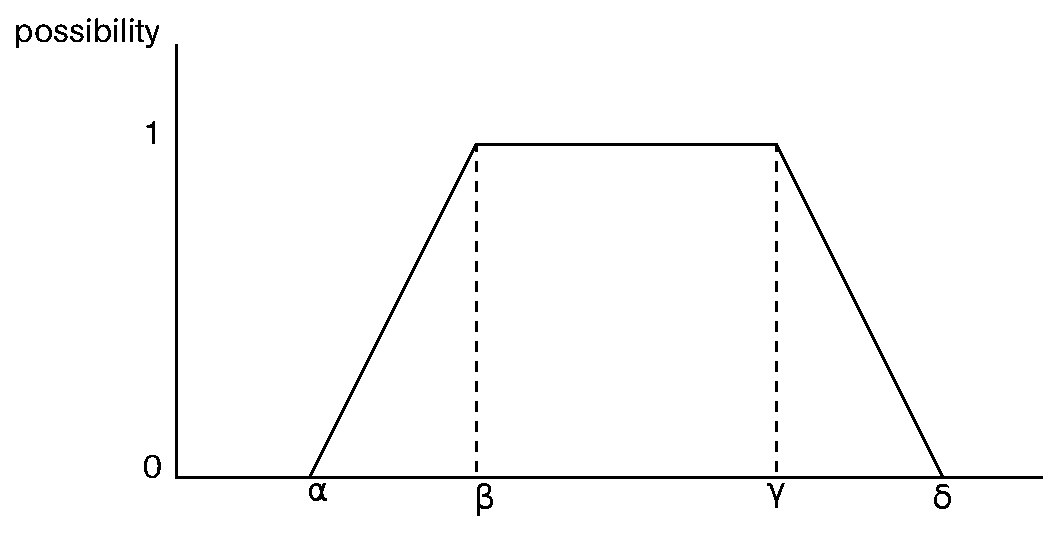
\includegraphics[scale=0.4]{graphs/trapezoidalDistribution.eps}
  \caption{Trapezoidal membership function}
  \label{fig:trapezoidal}
\end{figure}

The most convenient form of the membership function of a fuzzy number is a triangular function. It can be shown that such a membership function $\mu_M$ for a fuzzy number $M$ is convex and normalized. A visualization is given in figure \ref{fig:triangular}. Three reel values, denoted $a$, $b$ and $D$, suffice to represent a triangular membership function of a fuzzy number.
\begin{itemize}
\item
$D$ denotes the single value in the core of $M$
\item
$D-a$ is then $\inf \{u \in \mathbb{R} : \mu_{M}(u) > 0\}$
\item
$D+b$ is then $\sup \{u \in \mathbb{R} : \mu_{M}(u) > 0\}$
\end{itemize}
In this work, a fuzzy number defined as such will be noted as $\left[D, a, b \right]$.
\begin{figure}[h!]
  \centering
  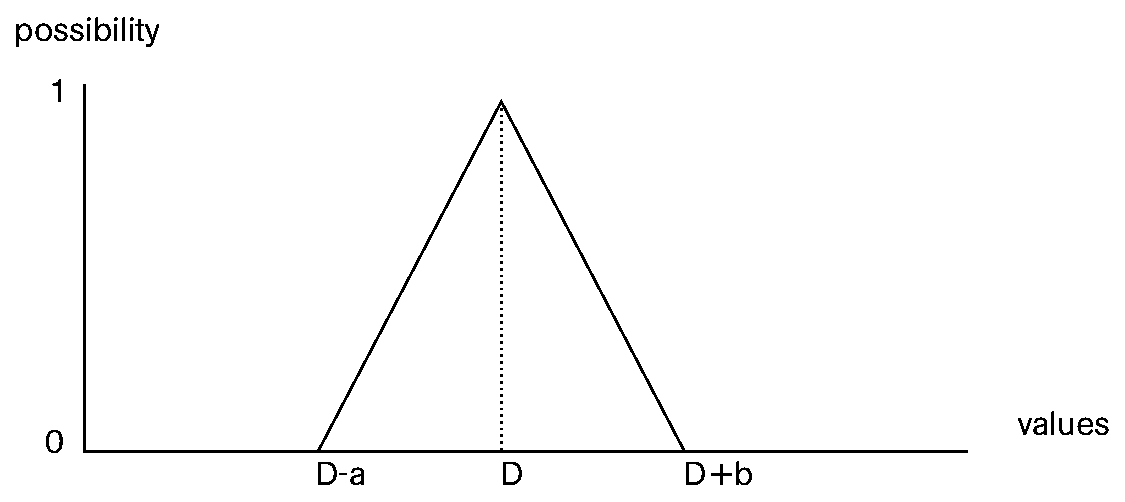
\includegraphics[scale=0.4]{graphs/triangular.eps}
  \caption{Triangular membership function.}
  \label{fig:triangular}
\end{figure}


%\subsubsection{Set evaluation by ill-known constraints}

\subsubsection{Interval Evaluation by Ill-known Constraints}
The problem of the interval evaluation is explained in \cite{Pon11}: for a crisp interval $I = \left[ a, b \right]$, the need exists to know if all points in this interval reside between the boundaries of the ill-known interval $\left[ X , Y \right]$, where $X,Y$ are ill-known values on the set of real numbers $\mathbb{R}$, and $\lambda$ is the evaluation function.

We assume that $X$ specifies the lower bound and $Y$ the upper bound for a given interval, we want to known whether all points in the interval are larger than or equal to $X$ and smaller than or equal to $Y$. Therefore, we consider two ill-known constraints:

\begin{eqnarray}
C_1\stackrel{\triangle}{=}\left(\leq,X\right)\\
C_2\stackrel{\triangle}{=}\left(\geq,Y\right).
\end{eqnarray}

The following expressions compute the possibility and the necessity: 

\begin{eqnarray}
\label{eq:interval-pos}
\Pos\left(\lambda([a,b])\right)=\\
\nonumber
\min\bigg(\sup_{a\geq w}\pi_{X}(w),\sup_{b\leq w}\pi_{Y}(w)\bigg)\\
\label{eq:interval-nec}
\Nec\left(\lambda([a,b])\right)=\\
\nonumber
\min\bigg(\inf_{a<w}1-\pi_{X}(w),\inf_{b>w}1-\pi_{Y}(w)\bigg).
\end{eqnarray}

%\paragraph{Example} Consider the ill-known values $X = \left[5, 2, 8\right]$ and $Y = \left[9, 7, 10 \right]$. The knowledge about the evaluation of the interval $\left[a, b \right]$  is given by the expressions \eqref{eq:interval-pos},\eqref{eq:interval-nec}.  Figure~\ref{fig:3d-possibility} shows a 3D plot of the possibility that an interval $[a,b]$ passes the evaluations specified by the ill-known constraints. Note the triangular form for the resulting possibility distribution since the condition $a \leq b$ holds.
%
%\begin{figure}[h!]
%\centering
%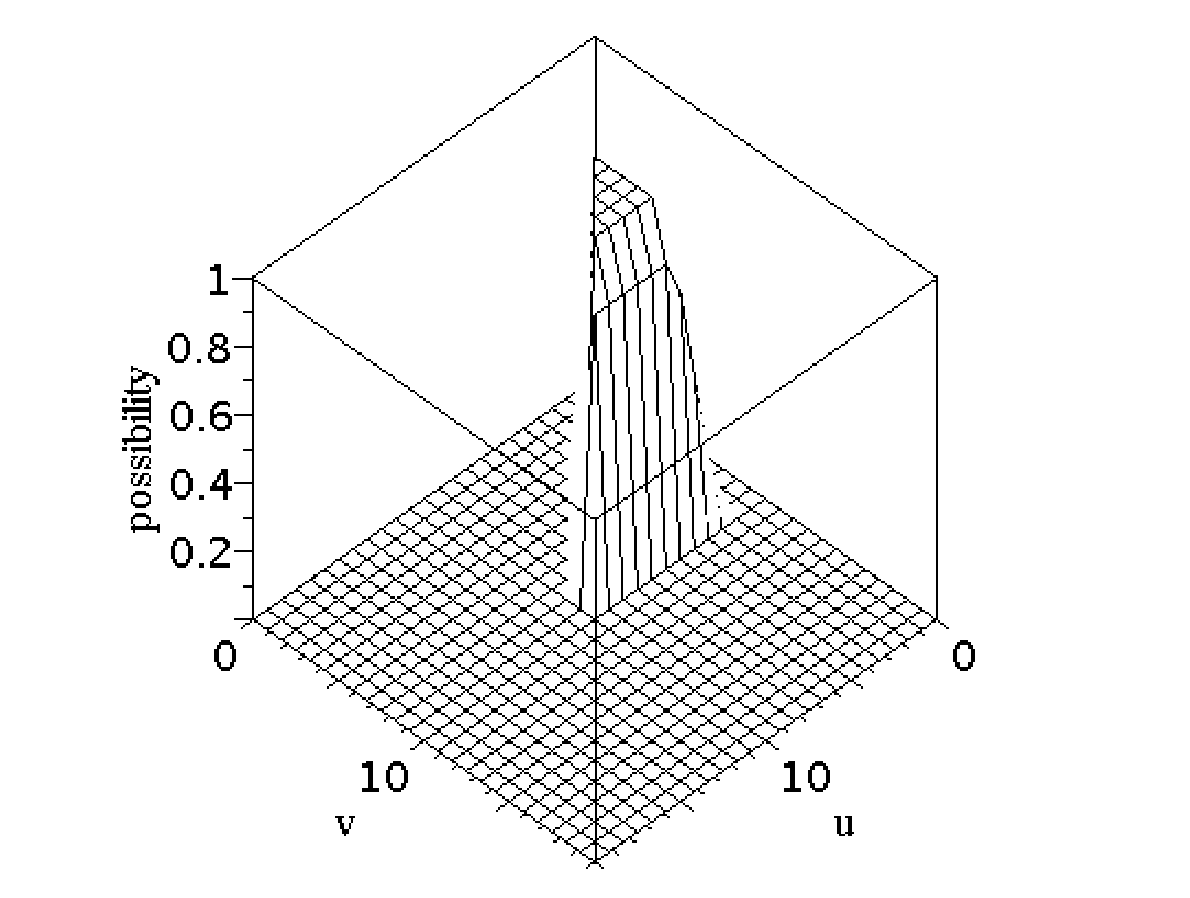
\includegraphics[scale=0.4]{graphs/3D_possibility.eps}
%\caption{Possibility of evaluation for the interval $[a,b]$.}
%\label{fig:3d-possibility}
%\end{figure}
%The necessity plot is obtained in a similar way and is shown in Figure~\ref{fig:3d-necessity}. Notice that the necessity measure is not normalized because the supports of $X$ and $Y$ overlap.
%\begin{figure}[h!]
%\centering
%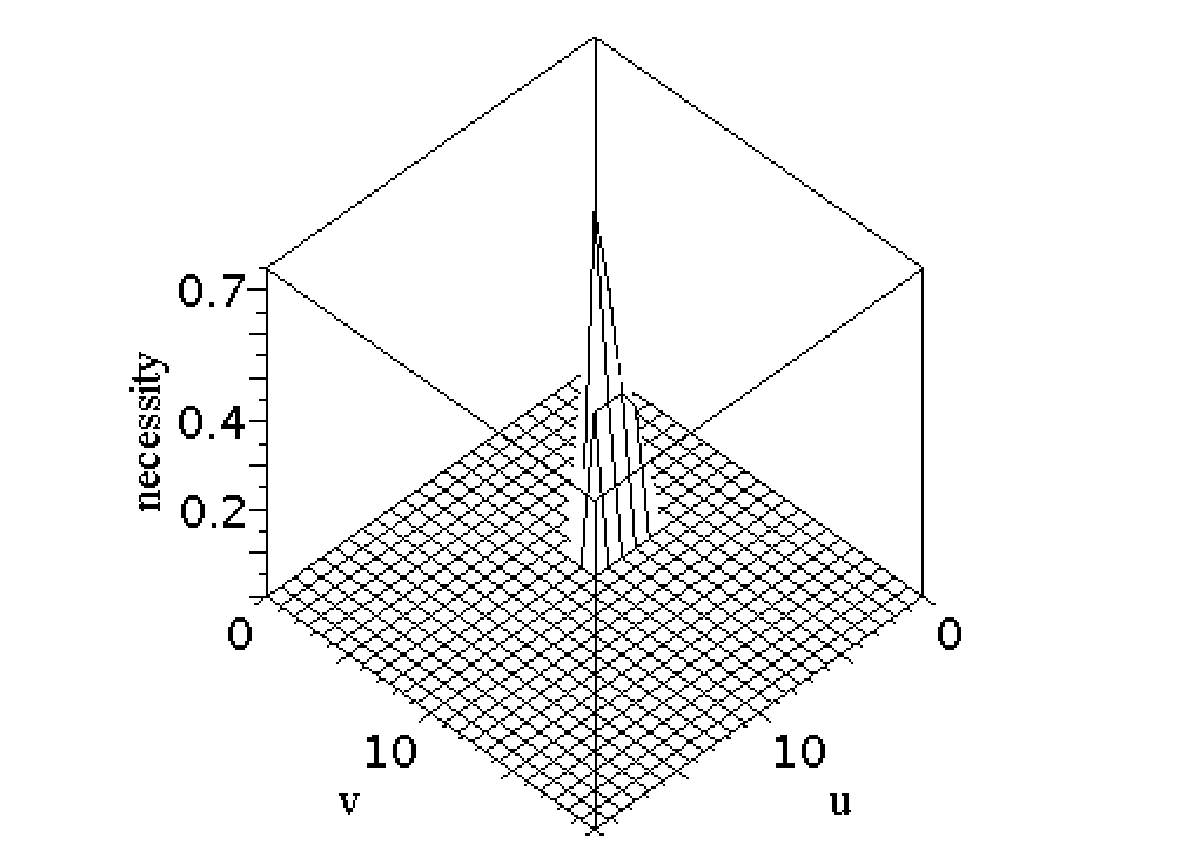
\includegraphics[scale=0.4]{graphs/3D_necessity.eps}
%\caption{Necessity of evaluation for the interval $[a,b]$.}
%\label{fig:3d-necessity}
%\end{figure}



\subsection{Temporal Databases}
%In this section, the proposed reasoning is applied to the specific context of intervals on the real line. This setting is of specific interest in the context of fuzzy temporal databases.
A temporal database \cite{Dyreson1994} is a database that manages some aspects of time in its schema. A \textbf{chronon} is the shortest duration of time supported by the database. The time can be represented either as points or intervals \cite{655777}. Fuzzy temporal models \cite{schockaert08} are proposed when the time points or intervals are not precisely known. There are proposals for the  fuzzyfication of the time point and the fuzzyfication of the time interval.\\
Allen \cite{Allen83} studied the comparison between two crisp time intervals. For fuzzy intervals, several proposals \cite{ohlbach04,nagypal03,schockaert08} have been done.


%Time granularity is also associated with the representation of the time. A granularity is the result of partitioning on the set of chronons. The conversion among granularities is a common issue within temporal databases \cite{Lin97efficientconversion}. Granularity is the basis of some systems \cite{Cru97},\cite{624013}.


Despite of user-defined time (an uninterpreted attribute; supported in the standard SQL2), there are 3 types of time in a temporal database:

\begin{itemize}
	\item
	\textbf{Transaction time}: The time when the fact is stored in the database.
	\item
	\textbf{Valid time}: The time when the fact is true in the modelled reality.
	\item
	\textbf{Decision time} \cite{Nascimento95}: The time when an event was decided to happen. 
	\end{itemize}
	
	 The  database model can be then classified into: transaction time \cite{Jensen91}, Valid time, bi-temporal \cite{Snodgrass84}(both valid and transaction time) or tri-temporal \cite{Nascimento95} (valid, transaction and decision time).

Fuzzy temporal models \cite{schockaert08} deal with time points \cite{Dubois89} or intervals \cite{Garrido2009} that are ill-known. Some fuzzy temporal models assume that the time stored in the database is an interval. The temporal interval is represented by two ill-known time points: $X$  an ill-known starting point and $Y$ an ill-known ending point. The interval $\left[X,Y\right]$ is not a fuzzy interval but an ill-known interval: it is a crisp interval but it is partially unknown which values are in this interval.
